\subsection{Experiment on Residue Correlation}
\label{subsec:exp:res}
\textbf{Inputs:}\\
We input a set of point clouds with the points consistently indexed respecting to their groundtruth correspondence, as shown in Figure~\ref{fig:input_for_exp_res}.\\
\begin{figure*}
	\centering
	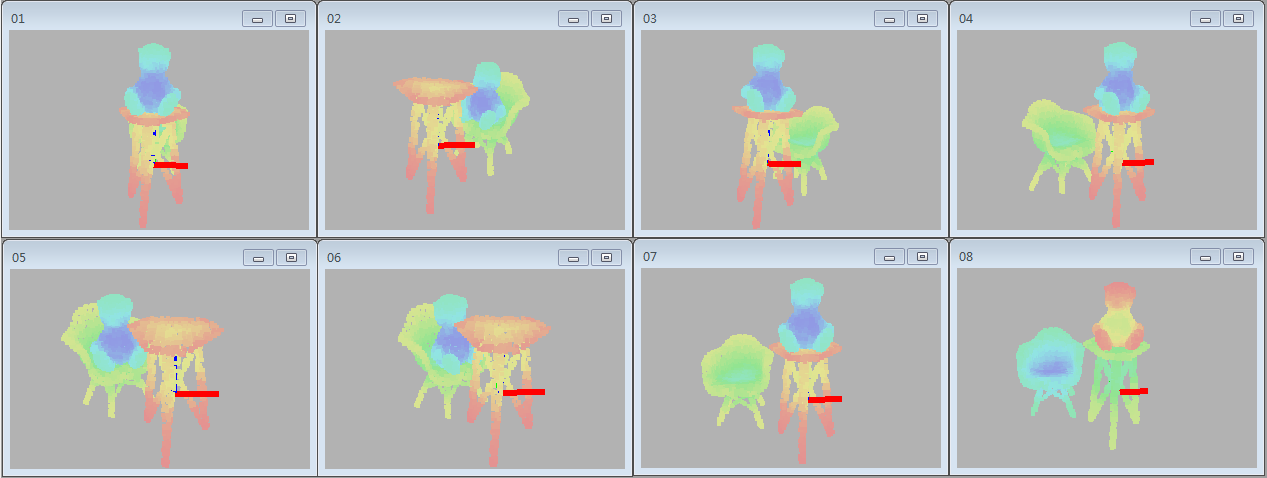
\includegraphics[width=\textwidth]{images/exp_res/inputs.png}
	\caption{Inputs of experiment on residue correlation: The points are colored by their index. From the color you should be able to see that: In frame 01 - 07, the points are indexed consistently respecting to object in order of table(1156 points), chair(1520 points), teddy(1351 points). In the frame 08, the points are indexed respecting to object in order of teddy, table, chair.}
	\label{fig:input_for_exp_res}
\end{figure*}
\textbf{Spectral Analysis:}\\
In order to do spectral analysis on point clouds, we first build supervoxels with \cite{Supervoxels} on point cloud and then construct a graph laplacian as a matrix $L=(a_{ij})$ defined by:
$$ a_{ij}=\left\{
\begin{aligned}
-\alpha d_{ij}-(1-\alpha) c_{ij} &~&if~i~and~j~is~an~edge\\
\sum\alpha d_{ij}+(1-\alpha) c_{ij} &~&if~i==j\\
0 &~&otherwise
\end{aligned}
\right.
$$
where $d_{ij}=\exp(\frac{-l_{ij}^2}{l_{mean}^2})$, $l_{ij}$ is the length of the edge in the graph of supervoxels and $\l_{mean}$ is average length of all edges.  $c_{ij}$ is the function indicating convexity of the edge and is defined as:
$$ c_{ij}=\left\{
\begin{aligned}
0 &~&if~\theta_{dif}<-\epsilon\\
1 &~&if~\theta_{dif}>\epsilon\\
\frac{\theta_{dif}}{2\epsilon}+\frac{1}{2} &~&otherwise
\end{aligned}
\right.
$$
where $\theta_{dif}=acos(<n_i,\frac{\overrightarrow{p_ip_j}}{||\overrightarrow{p_ip_j}||}>) - acos(<n_j,\frac{\overrightarrow{p_ip_j}}{||\overrightarrow{p_ip_j}||}>)$, in which the $\{n_i\}$ is the normal of supervoxels and $\{p_i\}$ is the center position of supervoxels. $\alpha$ is the weight between distance and convexity, for result in this paper we choose $\alpha=0.5$.\\
Based on the laplacian matrix we can get its eigenfunctions $\{\phi_n\}_{n=0...N}$ respecting to the N smallest eigenvalues $\lambda_0...\lambda_N$.\\ 
We can design an indicating function that maps each of the points to a unique real value. If we make this function "continue" respecting to the order of index, it can be constructed as the one shown in Figure~\ref{fig:indicating_function:a}.
\begin{figure}
\centering
\subfigure[]{
	\includegraphics[width=1\linewidth]{images/exp_res/indicator_00}
	\label{fig:indicating_function:a}
}
\subfigure[]{
	\includegraphics[width=1\linewidth]{images/exp_res/indicator_01}
	\label{fig:indicating_function:b}
	}
\subfigure[]{
	\includegraphics[width=1\linewidth]{images/exp_res/indicator_02}
	\label{fig:indicating_function:c}
}
\subfigure[]{
	\includegraphics[width=1\linewidth]{images/exp_res/indicator_03}
	\label{fig:indicating_function:d}
}
\subfigure[]{
	\includegraphics[width=1\linewidth]{images/exp_res/indicator_04}
	\label{fig:indicating_function:e}
}
\caption{Examples of indicating functions that is circularly shifted from the Figure~\ref{fig:indicating_function:a} respecting to the index order.}
\label{fig:indicating_function}
\end{figure}\\
For each point clouds, we project the indicating function $f$ onto the eigenfunctions by inner product and get coefficients: $\beta_n=<f,\phi_n>$. We choose $M$ coefficients with largest absolute values to reconstruct the indicating function: $\hat{f}=\sum_{i=1}^{M}\beta_{n_m}\phi_{n_m}$ and the residue function of the reconstruction $r=f-\hat{f}$. The results of inputs(Figure~\ref{fig:input_for_exp_res}) are shown in Figure~\ref{fig:res_for_exp_res}. In Figure~\ref{fig:res_for_exp_res}, the energy of residue functions are calculated as $E=\sum r^2$.
\begin{figure*}
	\centering
	\includegraphics[width=\textwidth]{images/exp_res/residue_all_s0}
	\caption{Residue functions of indicating functions: Each row is correspondent to a frame shown in Figure~\ref{fig:input_for_exp_res}. The first column is the spectrum of the indicating function. The Y axis is the value of coefficients and the X axis is the corresponding eigenvalue. The second column is the resconstructed indicating functions with M=30 absolute largest coefficients. The third column is the residue functions. The fourth column is the indicating functions.}
	\label{fig:res_for_exp_res}
\end{figure*}\\
We circularly shift the indicating functions as demonstrated in Figure~\ref{fig:indicating_function}. For each indicating function, we can calculate a residue energy. From Figure~\ref{fig:residue} we can see a clear similarity of the residue energy among the point clouds. 
\begin{figure*}
	\subfigure[When shift indicating functions with step = 2 we can get 2014 indicating functions and for each indicating function we can calculate a residue energy for reconstruction. We can see that though calculate independently on each point clouds, the residue energy have similar patterns.]{
		\includegraphics[width=0.49\textwidth]{images/exp_res/residue_energy}
		\label{fig:residue_energy}
	}
	\hspace{0.02\textwidth}
	\subfigure[To quatify the similar patterns of the residue energy. We first construct the median residue energy(Median Y) and then calculate the circular correlation between the residue energy and the Median Y. As we can see, when the point clouds are consistently indexed the max response appears near zero (circularly) as respect to frame 01 to 07, but the for frame 08 the max appears at the 1338 which is correspondent to 2676 considering the circulation has a step=2. This is exactly how much the index of frame 08 is shifted from the others.]{
		\includegraphics[width=0.49\textwidth]{images/exp_res/residue_correlation}
		\label{fig:residue_correlation}
	}
		\caption{Results of experiment on residue correlation}
		\label{fig:residue}
\end{figure*}